\section{HouseKeep}
\begin{frame}
\frametitle{講義概要}   

\underline{講義概要} \\
\ \\

微分・積分の基礎事項に関して講義する. 
微分は対象の変化を, 積分は対象の累積を解析する理論であり, データサイエンス, 経済学, 理工学など幅広い分野で基礎となる. 
実際, その強力な手法と幅広い応用ゆえ, 微分・積分は線形代数と合わせて大学数学の2本柱と位置付けられることが多い. 
本講義では, 一変数関数の微分・積分, 多項式近似, 多変数関数の微分・積分などを学習する. 



%\begin{enumerate}
%\item 関数, 極限, 微分, 接線, 極値問題, ..
%\item 高次微分, Taylor展開, 偏微分, ..
%\item 積分, 不定積分, 重積分, ..
%\end{enumerate}

%講義に\underline{計算用紙}と\underline{ペン}を持ってきて下さい!!

\end{frame}

\begin{slide}{スタッフ}
\begin{itemize}
\item 担当教員:環境情報学部 三次 仁(みつぎじん)mitsugi@keio.jp
\item SA:  瀧澤 将音 t21436mt@sfc.keio.ac.jp
\item SA: 柿本 嵩斗  s22197sk@sfc.keio.ac.jp
\item SA: 太田 侑吾 s21194yo@sfc.keio.ac.jp
\end{itemize}
基本、授業時間中に相談してください。授業時間外はK-LMSのmail機能でお願いします(SAにも通知されます)。
\end{slide}

\begin{slide}{授業の進め方}
\begin{itemize}
\item 授業の手法
\begin{itemize}
\item 基本的に講義が主体だが、適宜、演習を行う
\item 微分・積分の共通教材をベースに進めます。
\end{itemize}

\item 参考書

本授業の講義資料はだいたい次の本に基づく.
\begin{itemize}
\item 田澤義彦,しっかり学ぶ微分積分,東京電機大学出版局.
\end{itemize}
微分・積分に関す参考書・問題集は数多く出版されており、次はこの授業資料を作成する時にも参考にしている。
\begin{itemize}
\item 志賀浩二,微分・積分30講 (数学30講シリーズ),朝倉書店.
\item 志賀浩二,解析入門30講 (数学30講シリーズ),朝倉書店.
\item 杉浦光夫,解析入門Ⅰ(基礎数学2),東京大学出版会.
\end{itemize}
\end{itemize}
\end{slide}

\begin{slide}{成績評価など}
\begin{itemize}
\item 毎週課題(60\%)・授業内期末試験(40\%)を総合して評価します。
\item CNSメールや掲示(休講)を確認すること。
\item 剽窃や不正は厳しく罰せられます(今学期のすべての評語がDになる可能性があります)
\item ChatGPTなどのツールをうまく使いこなしましょう。得られた結果を自分なりに理解することがポイントです。(ネットで調べても友達に聞いても同じこと)。
\end{itemize}
\end{slide}

\begin{slide}{レポートの書き方}
\begin{itemize}
\item 締め切り後の提出は、基本ゼロ点です。
\item 答えを導けなくても、わからないところを明確にして提出てください。期限内提出であれば、よっぽどひどくなければゼロ点にはなりません。
\item overleafがお勧めです(授業でも簡単に解説します)。
\url{https://doratex.hatenablog.jp/entry/20180503/1525338512}
\item グラフは手書きでなくエクセルなどで描けるようになろう(授業でも簡単に解説します)。
\end{itemize}

\end{slide}
\begin{slide}{授業予定}
\begin{itemize}
\item 第1回 4/8 授業概要
\item 第2回 4/15	関数
\item 第3回 4/22 極限
\item 第4回 4/29 平均変化率・導関数(微分)
\item 第5回 5/13	様々な関数の微分
\item 第6回 5/20	逆関数、逆関数の微分
\item 第7回 5/27 接線・法線、ロピタルの定理
\item 第8回 6/3	高次導関数、テイラーの定理
\item 第9回 6/10 二変数関数、偏微分
\item 第10回 6/17 不定積分
\item 第11回 6/24 定積分
\item 第12回 7/1  多変数関数の積分
\item 第13回 7/8  総復習
\item 第14回 7/15  授業内試験
\end{itemize}
\end{slide}
%%%%%%%%%%%%%%%%%%%%%%%%%%%%%%%%%%%%%%%%%%%%%%%%%%%%%%%%%%%%%%%%%%%%%%%%%%%%%%%%%%%%%%%
%%%%%%%%%%%%%%%%%%%%%%%%%%%%%%%%%%%%%%%%%%%%%%%%%%%%%%%%%%%%%%%%%%%%%%%%%%%%%%%%%%%%%%%

%\begin{frame}
%\frametitle{参考書・成績評価・連絡先}  
%
%
%\underline{参考書} \\
%SOLにスライドをアップする.  
%自習用に参考書を一冊持っていると便利ですが, 必要ではありません. 
%例えば, 次のような教科書があります: 
%\begin{itemize}
%\item 志賀浩二, 微分・積分30講 (数学30講シリーズ), 朝倉書店. 
%\item 志賀浩二, 解析入門30講 (数学30講シリーズ), 朝倉書店. 
%\item 杉浦光夫, 解析入門I(基礎数学2), 東京大学出版会. 
%\end{itemize}
%\ \\
%
%
%\underline{成績評価} \\
%レポート2回60点 + 期末試験40点 \\
%(演習問題は提出不要) \\
%\ \\
%
%
%\underline{連絡先} \\
%atsushik@sfc.keio.ac.jp
%
%\end{frame}



%%%%%%%%%%%%%%%%%%%%%%%%%%%%%%%%%%%%%%%%%%%%%%%%%%%%%%%%%%%%%%%%%%%%%%%%%%%%%%%%%%%%%%%
%%%%%%%%%%%%%%%%%%%%%%%%%%%%%%%%%%%%%%%%%%%%%%%%%%%%%%%%%%%%%%%%%%%%%%%%%%%%%%%%%%%%%



%%%%%%%%%%%%%%%%%%%%%%%%%%%%%%%%%%%%%%%%%%%%%%%%%%%%%%%%%%%%%%%%%%%%%%%%%%%%%%%%%%%%%%%
%%%%%%%%%%%%%%%%%%%%%%%%%%%%%%%%%%%%%%%%%%%%%%%%%%%%%%%%%%%%%%%%%%%%%%%%%%%%%%%%%%%%%%%

\section{微分・積分とは何か?}


\begin{frame}
\frametitle{微分・積分とは何か?}


 \begin{figure}[htbp]
 \begin{center} 
  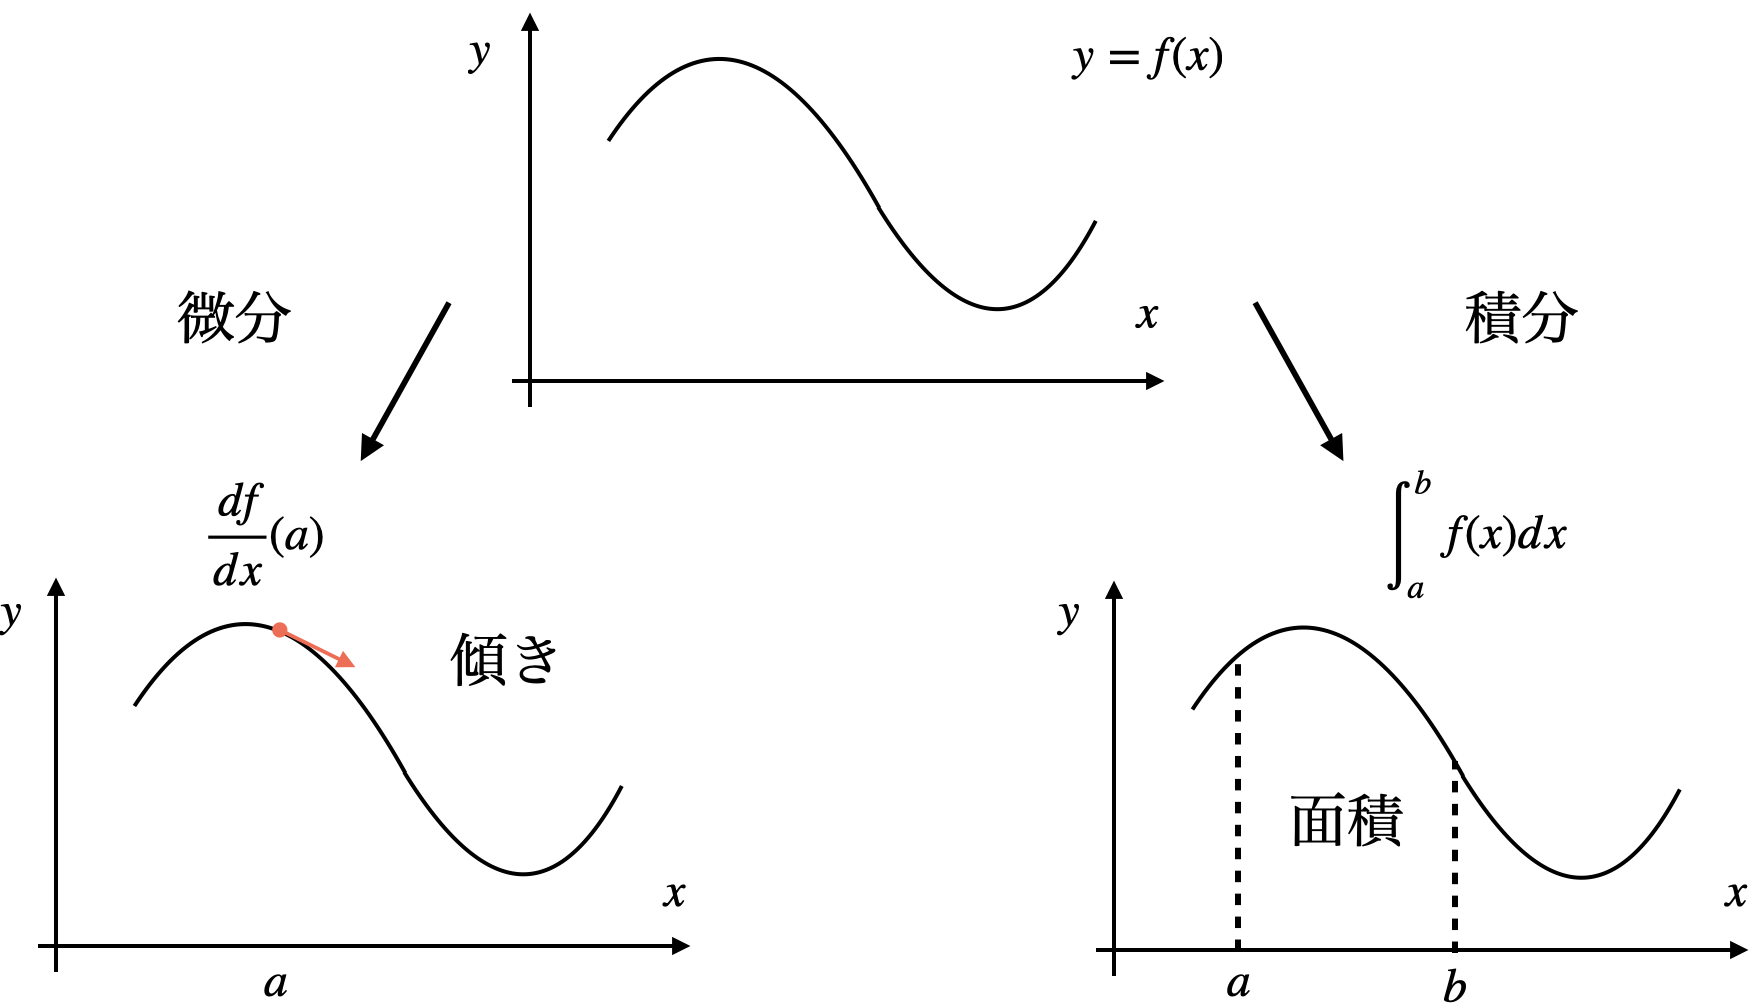
\includegraphics[width=100mm]{calculus1/diff_int.png}
 \end{center}
\end{figure}

\end{frame}


%%%%%%%%%%%%%%%%%%%%%%%%%%%%%%%%%%%%%%%%%%%%%%%%%%%%%%%%%%%%%%%%%%%%%%%%%%%%%%%%%%%%%%%
%%%%%%%%%%%%%%%%%%%%%%%%%%%%%%%%%%%%%%%%%%%%%%%%%%%%%%%%%%%%%%%%%%%%%%%%%%%%%%%%%%%%%%%


\begin{frame}
\frametitle{微分}

微分: 最も値の大きい・小さいところを探す方法

 \begin{figure}[htbp]
 \begin{center} 
  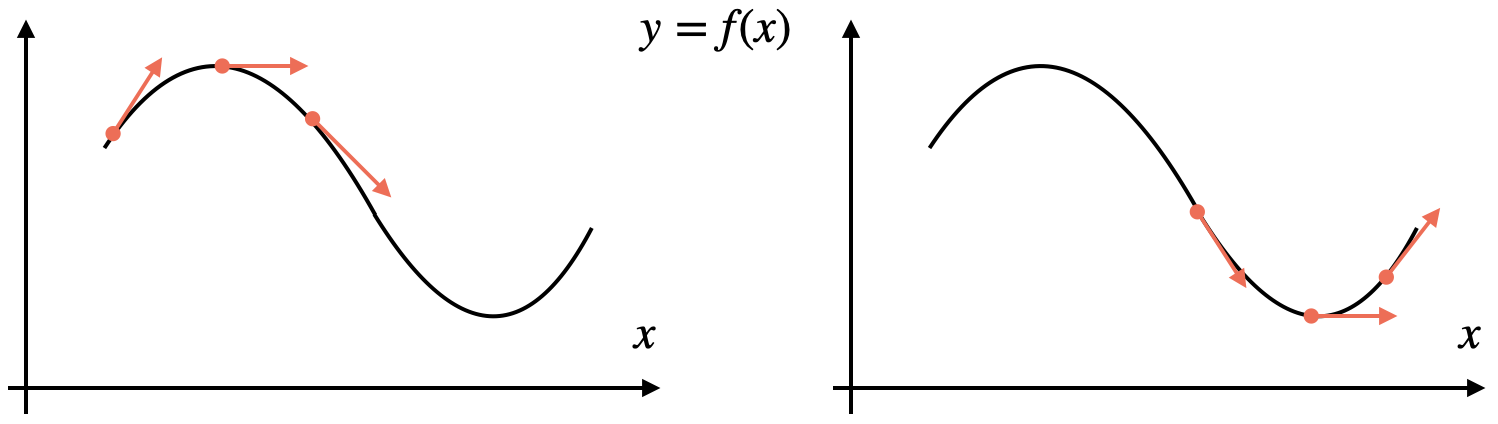
\includegraphics[width=100mm]{calculus1/diff.png}
 \end{center}
\end{figure}


\begin{itemize}
\item 極大点の頂上の手前では坂は上がり, 先では下る. 
\item 極小点の底の手前では坂は下り, 先では上がる. 
\item 極大点, 極小点 $\Rightarrow$ 傾き0. 
\item グラフの傾き = 関数の値の変化率, 未来の判断材料. 
\end{itemize}

\end{frame}


%%%%%%%%%%%%%%%%%%%%%%%%%%%%%%%%%%%%%%%%%%%%%%%%%%%%%%%%%%%%%%%%%%%%%%%%%%%%%%%%%%%%%%%
%%%%%%%%%%%%%%%%%%%%%%%%%%%%%%%%%%%%%%%%%%%%%%%%%%%%%%%%%%%%%%%%%%%%%%%%%%%%%%%%%%%%%%%


\begin{frame}
\frametitle{応用}   

最適化問題: 適当な条件を満たす最適解を探す

\begin{itemize}
\item 等周問題: 周の長さが$l$の長方形の中で面積を最大にするものは? 
\item 面積$A(x)=x(l/2-x)$
\end{itemize}

 \begin{figure}[htbp]
 \begin{center} 
  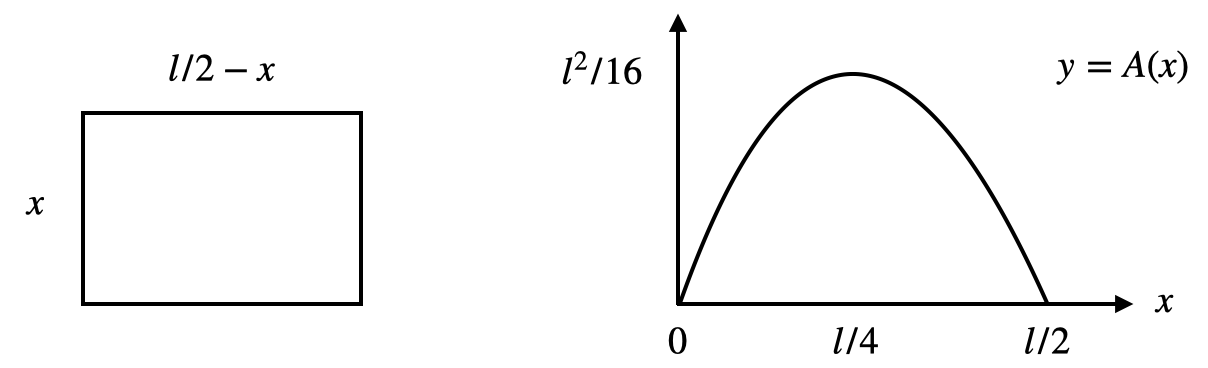
\includegraphics[width=100mm]{calculus1/LecArea.png}
 \end{center}
\end{figure}

\end{frame}


%%%%%%%%%%%%%%%%%%%%%%%%%%%%%%%%%%%%%%%%%%%%%%%%%%%%%%%%%%%%%%%%%%%%%%%%%%%%%%%%%%%%%%%
%%%%%%%%%%%%%%%%%%%%%%%%%%%%%%%%%%%%%%%%%%%%%%%%%%%%%%%%%%%%%%%%%%%%%%%%%%%%%%%%%%%%%%%


\begin{frame}
\frametitle{積分}

積分: これまでの蓄積を計算する方法

 \begin{figure}[htbp]
 \begin{center} 
  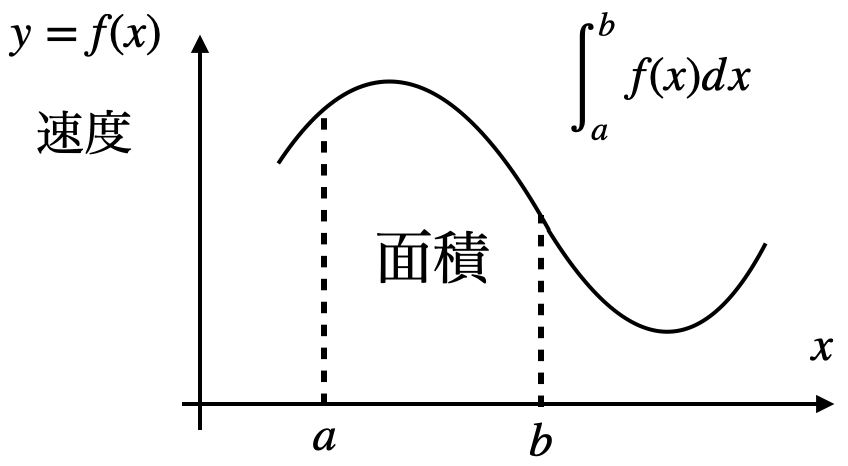
\includegraphics[width=60mm]{calculus1/int_speed.png}
 \end{center}
\end{figure}


\begin{itemize}
\item 面積$\int_a^b f(x)dx$は時刻$a$から時刻$b$までに移動した距離. 
\item 平均速度 = 面積/時間. 
\item 面積 = 過去の蓄積, 過去の判断材料.
\end{itemize}

\end{frame}


%%%%%%%%%%%%%%%%%%%%%%%%%%%%%%%%%%%%%%%%%%%%%%%%%%%%%%%%%%%%%%%%%%%%%%%%%%%%%%%%%%%%%%%
%%%%%%%%%%%%%%%%%%%%%%%%%%%%%%%%%%%%%%%%%%%%%%%%%%%%%%%%%%%%%%%%%%%%%%%%%%%%%%%%%%%%%%%


\begin{frame}
\frametitle{積分}

時刻$a$から時刻$t$までに移動した距離は$F(t)=\int_a^tf(x)dx$で与えられた. 

 \begin{figure}[htbp]
 \begin{center} 
  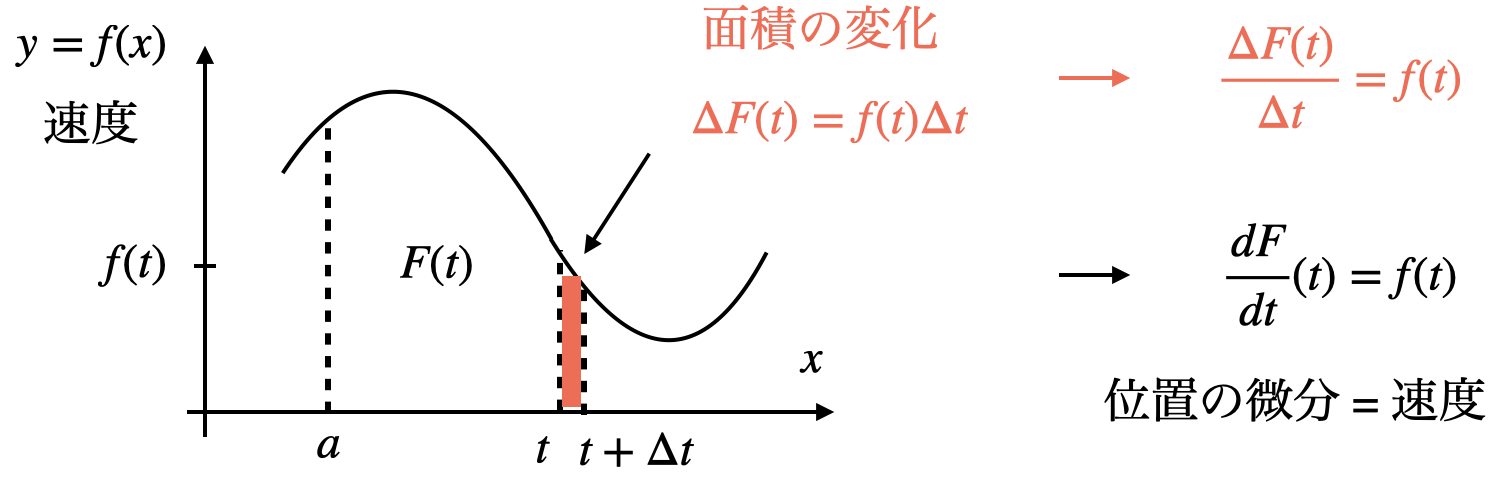
\includegraphics[width=100mm]{calculus1/diff_pos=speed.png}
 \end{center}
\end{figure}


\begin{itemize}
\item 「速度」を積分すると「位置」(過去の蓄積). 
\item 「位置」を微分すると「速度」(現在の変化). 
\item  一般に, 微分と積分は逆操作. 
\end{itemize}

\end{frame}



%%%%%%%%%%%%%%%%%%%%%%%%%%%%%%%%%%%%%%%%%%%%%%%%%%%%%%%%%%%%%%%%%%%%%%%%%%%%%%%%%%%%%%%
%%%%%%%%%%%%%%%%%%%%%%%%%%%%%%%%%%%%%%%%%%%%%%%%%%%%%%%%%%%%%%%%%%%%%%%%%%%%%%%%%%%%%%%



\begin{frame}
\frametitle{微分・積分}

以上を簡単にまとめると

 \begin{figure}[htbp]
 \begin{center} 
  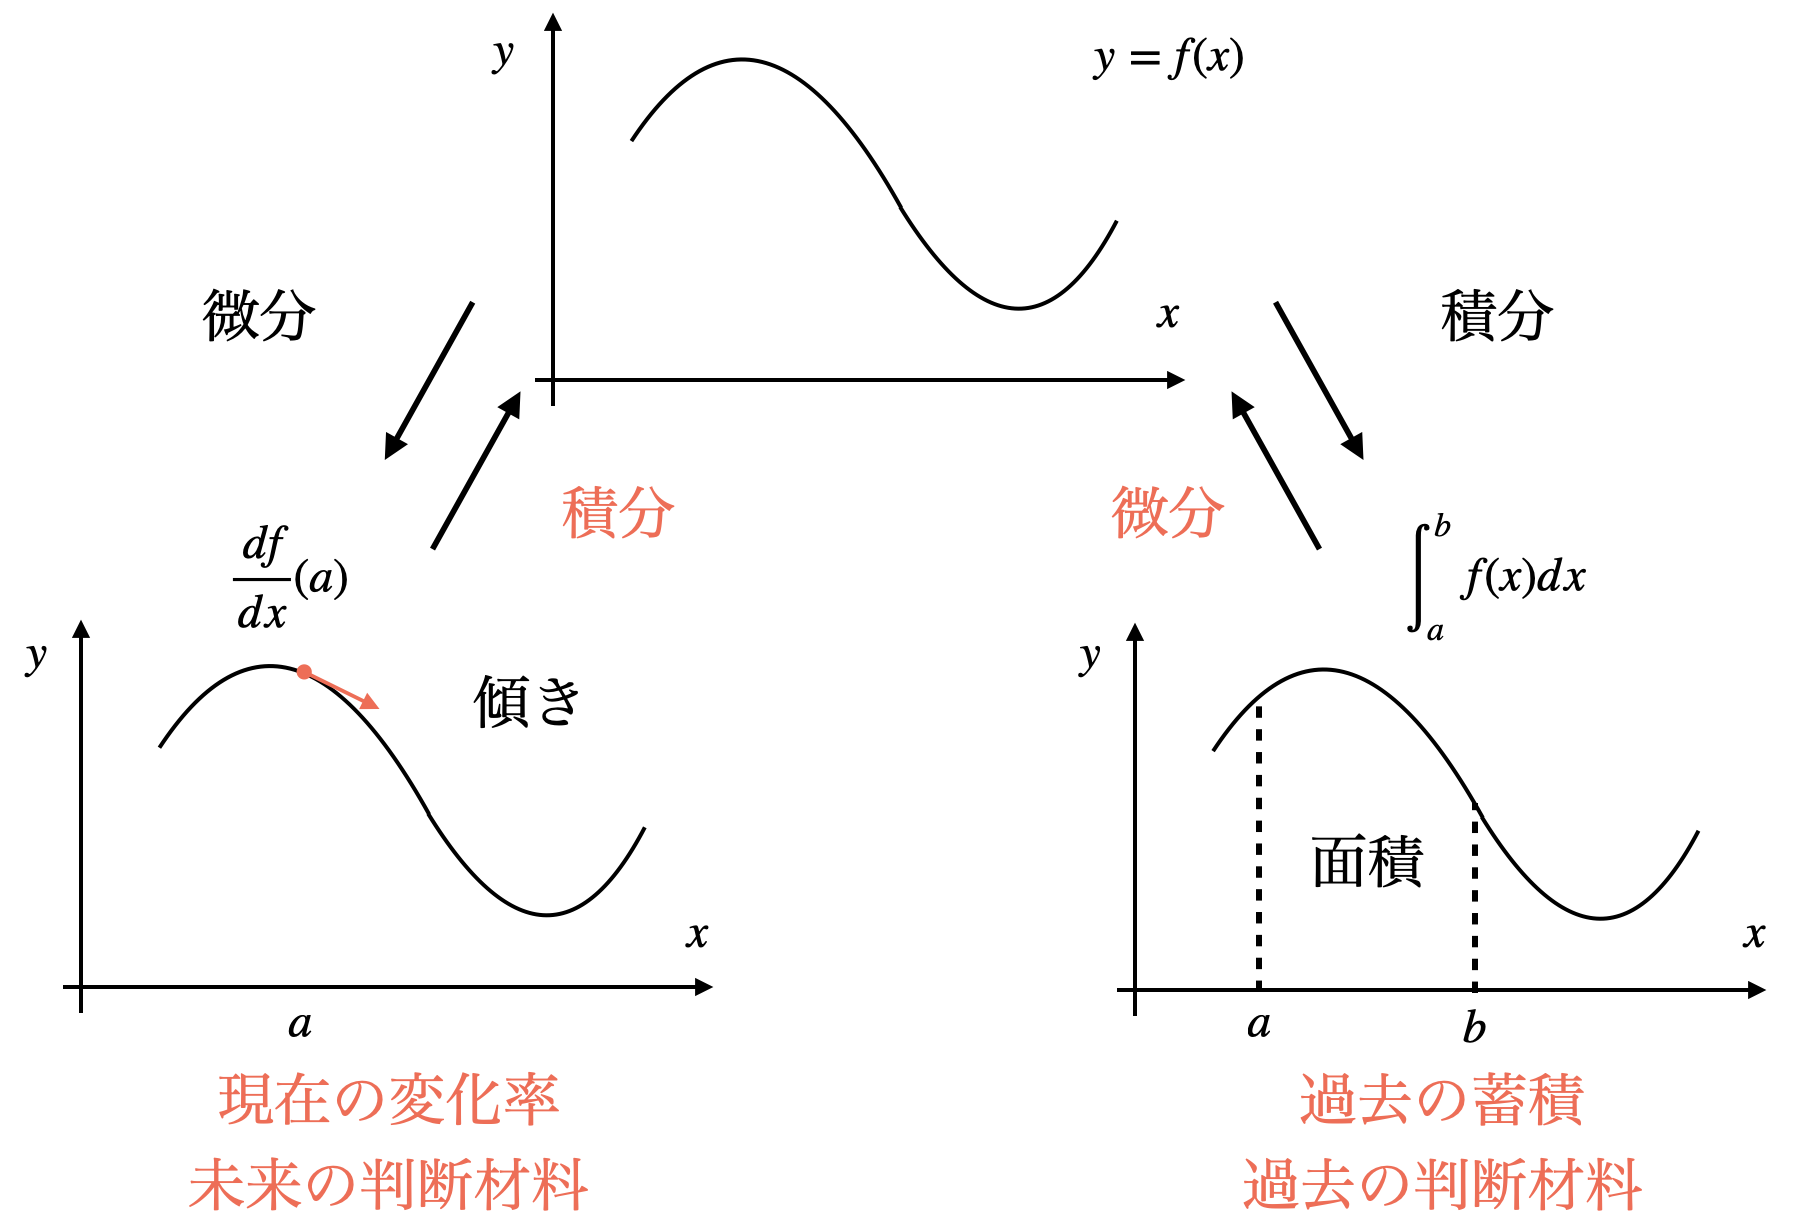
\includegraphics[width=100mm]{calculus1/diff_int2.png}
 \end{center}
\end{figure}

\end{frame}
\begin{slide}{課題\#1}
\begin{itemize}
\item 微分・積分が今後自分のキャリアにどのように役立ちそうか、今日の講義も踏まえて、考えを述べなさい。もしどうしても考えているキャリアに役立つと思えない場合には、その理由をまとめること
\item 授業に関する期待や要望などがあれば、それも含めること。採点対象外。
\item A4 1枚以内。PDFでKLMSに提出。
\end{itemize}

\end{slide}



